\section{Vector fields}

\begin{frame}{Vector fields}
\begin{columns}
\begin{column}{0.7\textwidth}
Let \( T:\mm\to BS^1 \) be an oriented tangent bundle on a 2-dim realization of a combinatorial manifold.
\begin{itemize}
\item Our bundles of mere circles can only model \alert{nonzero} tangent vectors.
\item  A global section of this family would be a trivialization of \( T \), so that's not a good definition.
\end{itemize}
\quad\\~\\
\onslide<2->{
Our solution:
\begin{itemize}
\item<3-> A \alert{vector field} is a term \alert{\( X:\pit{m:\mm_1}Tm \)}.
\item<4-> It models a classical \alert{nonvanishing} vector field on the 1-skeleton.
\item<5-> We model classical zeros by omitting the faces.
\end{itemize}
}
\end{column}
\begin{column}{0.3\textwidth}
% https://q.uiver.app/#q=WzAsMyxbMSwxLCJCU14xIl0sWzEsMCwiKiJdLFswLDEsIlxcbW0iXSxbMiwwLCJUIiwyXSxbMiwxLCJYIiwwLHsic3R5bGUiOnsiYm9keSI6eyJuYW1lIjoiZGFzaGVkIn19fV0sWzEsMCwie1NeMX0iXV0=
\[\begin{tikzcd}[ampersand replacement=\&]
  \& {*} \\
  \mm \& {BS^1}
  \arrow["{{S^1}}", from=1-2, to=2-2]
  \arrow["X", dashed, from=2-1, to=1-2]
  \arrow["T"', from=2-1, to=2-2]
\end{tikzcd}\]
\onslide<2->{\begin{tikzpicture}%
  [x={(-0.860769cm, -0.121512cm)},
  y={(0.508996cm, -0.205391cm)},
  z={(-0.000053cm, 0.971107cm)},
  scale=1,
  back/.style={loosely dotted, thin},
  edge/.style={black, thick},
  arrow/.style={black, very thick, solid, -{Stealth[scale=0.8]}},
  facet/.style={fill=blue!95!black,fill opacity=0.0},
  vertex/.style={inner sep=1pt,circle,draw=green!25!black,fill=black,thick}]
%% Drawing the vertices in the front
%%
\begin{scope}[nodes=vertex]
\node[label=above right:\( b \)] at (-1, 1, 0) (b)     {};
\node[label=below:\( y \)] at (0, 0, -1.4) (y)    {};
\node[label=above:\( w \)] at (0, 0, 1.4)  (w)   {};
\node[label=above left:\( g \)] at (1, -1, 0) (g)    {};
\node[label=above left:\( r \)] at (1, 1, 0)  (r)   {};
\node[label=above right:\( o \)] at (-1, -1, 0) (o)    {};
\end{scope}
%% Drawing edges in the back
%%
\draw[edge,back,arrow] (o) -- (b);
\draw[edge,back,arrow] (y) -- (o);
\draw[edge,back] (o) -- (w);
\draw[edge,back] (o) -- (g);
%% Drawing vertices in the back
%%
\node[vertex] at (o)     {};
%% Drawing the facets
%%
\fill[facet] (1, 1, 0) -- (0, 0, -1.4) -- (1, -1, 0) -- cycle {};
\fill[facet] (1, 1, 0) -- (0, 0, 1.4) -- (1, -1, 0) -- cycle {};
\fill[facet] (1, 1, 0) -- (-1, 1, 0) -- (0, 0, 1.4) -- cycle {};
\fill[facet] (1, 1, 0) -- (-1, 1, 0) -- (0, 0, -1.4) -- cycle {};
%% Drawing edges in the front
%%
\draw[edge,arrow] (b) -- (y);
\draw[edge] (b) -- (w);
\draw[edge] (b) -- (r);
\draw[edge] (y) -- (g);
\draw[edge] (y) -- (r);
\draw[edge,arrow] (g) -- (w);
\draw[edge,arrow] (w) -- (r);
\draw[edge,arrow] (r) -- (g);
\end{tikzpicture}
}
\end{column}
\end{columns}
\end{frame}

\begin{frame}{Reminder: pathovers}
\begin{columns}
\begin{column}{0.35\textwidth}
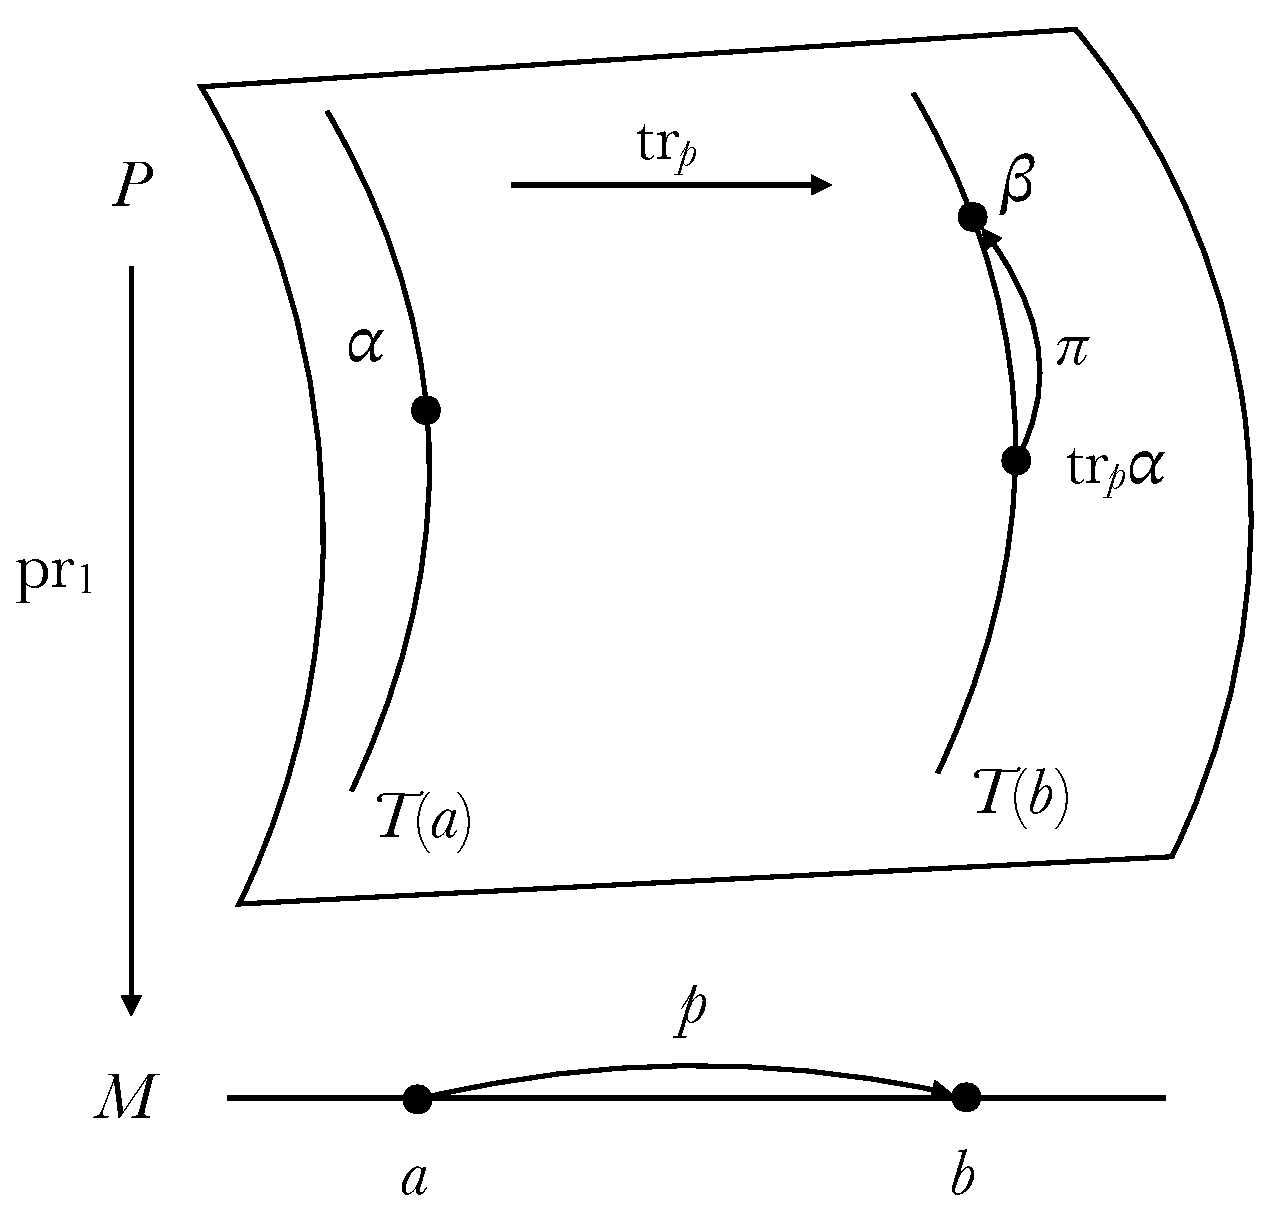
\includegraphics[width=30ex]{figs/pathovers.pdf}
\end{column}
\begin{column}{0.65\textwidth}
\begin{itemize}
\item Recall pathovers (dependent paths).
\item There is an asymmetry: we pick a fiber to display \( \pi \), the path over \( p \).
\item Dependent functions map paths to pathovers: \( \apd (X)(p):\tr_p(X(a))=X(b) \) (simply denoted \( X(p) \)).
\end{itemize}
\end{column}
\end{columns}
\end{frame}

\begin{frame}
Next goal: define the index of a vector field on a face by computing \( X(\partial F) \) around a face.
\end{frame}

\begin{frame}
\begin{columns}
\begin{column}{0.65\textwidth}
\vspace{12pt}
\begingroup
\tikzset{every picture/.style={scale=0.85}}
\begin{tikzpicture}
  [arrow/.style={-{Stealth[scale=1.1]}}, vec/.style={ultra thick, color=black}, vectr/.style={thick, color=black}, vectrtr/.style={thick, dashed, color=black}, vectrtrtr/.style={thick, dotted, color=black}]
  \tikzset{oo/.style={circle, scale=0.6, fill=black}}
  \tikzset{ii/.style={circle, scale=0.3, fill=gray}}
\newlength{\mylen}
  \setlength{\mylen}{3cm}
  \newlength{\mylin}
  \setlength{\mylin}{0.5cm}
    \node[oo, label=below:\( v_1 \)] (V1) at (0, 0) {};
    \node[oo, label=below:\( v_2 \)] (V2) at (2*\mylen, 0) {};
    \node[oo, label=above:\( v_3 \)] (V3) at (\mylen, 1.732*\mylen) {};

    \draw[arrow] (V2) edge[very thick, color=teal, "\( e_{23} \)"] (V3);
    \draw[arrow] (V1) edge[very thick, color=magenta, "\( e_{12} \)"] (V2);
    \draw[arrow] (V3) edge[very thick, color=blue, "\( e_{31} \)"] (V1);
    
    \node [left=1.3\mylin of  V1,  label=center:\( T_1 \)] {};
    \node [right=1.3\mylin of  V2,  label=center:\( T_2 \)] {};
    \node [left=1.3\mylin of  V3,  label=center:\( T_3 \)] {};

\end{tikzpicture}

\endgroup
\end{column}
\begin{column}{0.35\textwidth}
An example of \alert{swirling} and \alert{index} at this face.
\end{column}
\end{columns}
\end{frame}

\begin{frame}
\begin{columns}
\begin{column}{0.65\textwidth}
\vspace{12pt}
\begingroup
\tikzset{every picture/.style={scale=0.85}}
\begin{tikzpicture}
  [arrow/.style={-{Stealth[scale=1.1]}}, vec/.style={ultra thick, color=black}, vectr/.style={thick, color=black}, vectrtr/.style={thick, dashed, color=black}, vectrtrtr/.style={thick, dotted, color=black}]
  \tikzset{oo/.style={circle, scale=0.6, fill=black}}
  \tikzset{ii/.style={circle, scale=0.3, fill=gray}}
  \setlength{\mylen}{3cm}
  \setlength{\mylin}{1.2cm}
    \node[oo, label=below right:\( v_1 \)] (V1) at (0, 0) {};
    \node[oo, label=below:\( v_3 \)] (V3) at (2*\mylen, 0) {};
    \node[oo, label=above:\( v_2 \)] (V2) at (\mylen, 1.732*\mylen) {};

    \draw[arrow] (V2) edge[very thick, color=teal, "\( e_{23} \)"] (V3);
    \draw[arrow] (V1) edge[very thick, color=magenta, "\( e_{12} \)"] (V2);
    \draw[arrow] (V3) edge[very thick, color=blue, "\( e_{31} \)"] (V1);
    
    \node [ii, above right=\mylin of V1] (V11) {};
    \node [ii, below right=\mylin of V1] (V14) {};
    \node [ii, below left=\mylin of  V1] (V13) {};
    \node [ii, above left= \mylin of V1] (V12) {};

    \node [left=1.3\mylin of  V1,  label=center:\( T_1 \)] {};
    \node [right=1.3\mylin of  V2,  label=center:\( T_2 \)] {};
    \node [right=1.3\mylin of  V3,  label=center:\( T_3 \)] {};

    \node [ii, above right=\mylin of V2] (V21) {};
    \node [ii, below right=\mylin of V2] (V24) {};
    \node [ii, below left=\mylin of  V2] (V23) {};
    \node [ii, above left= \mylin of V2] (V22) {};

    \node [ii, above right=\mylin of V3] (V31) {};
    \node [ii, below right=\mylin of V3] (V34) {};
    \node [ii, below left=\mylin of  V3] (V33) {};
    \node [ii, above left= \mylin of V3] (V32) {};

    \draw[dashed] (V11) -- (V12);
    \draw[dashed] (V12) -- (V13);
    \draw[dashed] (V13) -- (V14);
    \draw[dashed] (V14) -- (V11);

    \draw[dashed] (V21) -- (V22);
    \draw[dashed] (V22) -- (V23);
    \draw[dashed] (V23) -- (V24);
    \draw[dashed] (V24) -- (V21);
    
    \draw[dashed] (V31) -- (V32);
    \draw[dashed] (V32) -- (V33);
    \draw[dashed] (V33) -- (V34);
    \draw[dashed] (V34) -- (V31);
    
    \draw[arrow] (V1) edge[vec] (V11);
\end{tikzpicture}

\endgroup
\end{column}
\begin{column}{0.35\textwidth}
An example of \alert{swirling} and \alert{index} at this face.
\begin{itemize}
\item<1-> Denote by \( X_1 \) this vector \( X(v_1):T_1 \).
\item<1-> \phantom{Say \( T_{21} \) is trivial. Denote the transported vector as thinner.}
\item<1-> \phantom{Say \( T_{32} \) rotates clockwise. Denote the twice-transported vector as dashed.}
\item<1-> \phantom{Say \( T_{13} \) is trivial. The thrice-transported vecor is dotted.}
\end{itemize}
\end{column}
\end{columns}
\end{frame}

\begin{frame}
\begin{columns}
\begin{column}{0.65\textwidth}
\vspace{12pt}
\begingroup
\tikzset{every picture/.style={scale=0.85}}
\begin{tikzpicture}
  [arrow/.style={-{Stealth[scale=1.1]}}, vec/.style={ultra thick, color=black}, vectr/.style={thick, color=black}, vectrtr/.style={thick, dashed, color=black}, vectrtrtr/.style={thick, dotted, color=black}]
  \tikzset{oo/.style={circle, scale=0.6, fill=black}}
  \tikzset{ii/.style={circle, scale=0.3, fill=gray}}
  \setlength{\mylen}{3cm}
  \setlength{\mylin}{1.2cm}
    \node[oo, label=below right:\( v_1 \)] (V1) at (0, 0) {};
    \node[oo, label=below:\( v_2 \)] (V2) at (2*\mylen, 0) {};
    \node[oo, label=above:\( v_3 \)] (V3) at (\mylen, 1.732*\mylen) {};

    \draw[arrow] (V2) edge[very thick, color=teal, "\( e_{23} \)"] (V3);
    \draw[arrow] (V1) edge[very thick, color=magenta, "\( e_{12} \)"] (V2);
    \draw[arrow] (V3) edge[very thick, color=blue, "\( e_{31} \)"] (V1);
    
    \node [ii, above right=\mylin of V1] (V11) {};
    \node [ii, below right=\mylin of V1] (V12) {};
    \node [ii, below left=\mylin of  V1] (V13) {};
    \node [ii, above left= \mylin of V1] (V14) {};

    \node [left=1.3\mylin of  V1,  label=center:\( T_1 \)] {};
    \node [right=1.3\mylin of  V2,  label=center:\( T_2 \)] {};
    \node [left=1.3\mylin of  V3,  label=center:\( T_3 \)] {};

    \node [ii, above right=\mylin of V2] (V21) {};
    \node [ii, below right=\mylin of V2] (V22) {};
    \node [ii, below left=\mylin of  V2] (V23) {};
    \node [ii, above left= \mylin of V2] (V24) {};

    \node [ii, above right=\mylin of V3] (V31) {};
    \node [ii, below right=\mylin of V3] (V32) {};
    \node [ii, below left=\mylin of  V3] (V33) {};
    \node [ii, above left= \mylin of V3] (V34) {};

    \draw[dashed] (V11) -- (V12);
    \draw[dashed] (V12) -- (V13);
    \draw[dashed] (V13) -- (V14);
    \draw[dashed] (V14) -- (V11);

    \draw[dashed] (V21) -- (V22);
    \draw[dashed] (V22) -- (V23);
    \draw[dashed] (V23) -- (V24);
    \draw[dashed] (V24) -- (V21);
    
    \draw[dashed] (V31) -- (V32);
    \draw[dashed] (V32) -- (V33);
    \draw[dashed] (V33) -- (V34);
    \draw[dashed] (V34) -- (V31);
    
    \draw[arrow] (V1) edge[vec] (V11);
    \draw[arrow] (V2) edge[vectr] (V21);
\end{tikzpicture}

\endgroup
\end{column}
\begin{column}{0.35\textwidth}
An example of \alert{swirling} and \alert{index} at this face.
\begin{itemize}
\item<1-> Denote by \( X_1 \) this vector \( X(v_1):T_1 \).
\item<1-> Say \( T_{21} \) is trivial. Denote the transported vector as thinner.
\item<1-> \phantom{Say \( T_{32} \) rotates clockwise. Denote the twice-transported vector as dashed.}
\item<1-> \phantom{Say \( T_{13} \) is trivial. The thrice-transported vecor is dotted.}
\end{itemize}
\end{column}
\end{columns}
\end{frame}

\begin{frame}
\begin{columns}
\begin{column}{0.65\textwidth}
\vspace{12pt}
\begingroup
\tikzset{every picture/.style={scale=0.85}}
\begin{tikzpicture}
  [arrow/.style={-{Stealth[scale=1.1]}}, vec/.style={ultra thick, color=black}, vectr/.style={thick, color=black}, vectrtr/.style={thick, dashed, color=black}, vectrtrtr/.style={thick, dotted, color=black}]
  \tikzset{oo/.style={circle, scale=0.6, fill=black}}
  \tikzset{ii/.style={circle, scale=0.3, fill=gray}}
  \setlength{\mylen}{3cm}
  \setlength{\mylin}{1.2cm}
    \node[oo, label=below right:\( v_1 \)] (V1) at (0, 0) {};
    \node[oo, label=below:\( v_3 \)] (V3) at (2*\mylen, 0) {};
    \node[oo, label=above:\( v_2 \)] (V2) at (\mylen, 1.732*\mylen) {};

    \draw[arrow] (V2) edge[very thick, color=teal, "\( e_{23} \)"] (V3);
    \draw[arrow] (V1) edge[very thick, color=magenta, "\( e_{12} \)"] (V2);
    \draw[arrow] (V3) edge[very thick, color=blue, "\( e_{31} \)"] (V1);
    
    \node [ii, above right=\mylin of V1] (V11) {};
    \node [ii, below right=\mylin of V1] (V14) {};
    \node [ii, below left=\mylin of  V1] (V13) {};
    \node [ii, above left= \mylin of V1] (V12) {};

    \node [left=1.3\mylin of  V1,  label=center:\( T_1 \)] {};
    \node [right=1.3\mylin of  V2,  label=center:\( T_2 \)] {};
    \node [right=1.3\mylin of  V3,  label=center:\( T_3 \)] {};

    \node [ii, above right=\mylin of V2] (V21) {};
    \node [ii, below right=\mylin of V2] (V24) {};
    \node [ii, below left=\mylin of  V2] (V23) {};
    \node [ii, above left= \mylin of V2] (V22) {};

    \node [ii, above right=\mylin of V3] (V31) {};
    \node [ii, below right=\mylin of V3] (V34) {};
    \node [ii, below left=\mylin of  V3] (V33) {};
    \node [ii, above left= \mylin of V3] (V32) {};

    \draw[dashed] (V11) -- (V12);
    \draw[dashed] (V12) -- (V13);
    \draw[dashed] (V13) -- (V14);
    \draw[dashed] (V14) -- (V11);

    \draw[dashed] (V21) -- (V22);
    \draw[dashed] (V22) -- (V23);
    \draw[dashed] (V23) -- (V24);
    \draw[dashed] (V24) -- (V21);
    
    \draw[dashed] (V31) -- (V32);
    \draw[dashed] (V32) -- (V33);
    \draw[dashed] (V33) -- (V34);
    \draw[dashed] (V34) -- (V31);
    
    \draw[arrow] (V1) edge[vec] (V11);
    \draw[arrow] (V2) edge[vectr] (V21);
    \draw[arrow] (V3) edge[vectrtr] (V34);
\end{tikzpicture}

\endgroup
\end{column}
\begin{column}{0.35\textwidth}
An example of \alert{swirling} and \alert{index} at this face.
\begin{itemize}
\item<1-> Denote by \( X_1 \) this vector \( X(v_1):T_1 \).
\item<1-> Say \( T_{21} \) is trivial. Denote the transported vector as thinner.
\item<1-> Say \( T_{32} \) rotates clockwise. Denote the twice-transported vector as dashed.
\item<1-> \phantom{Say \( T_{13} \) is trivial. The thrice-transported vecor is dotted.}
\end{itemize}
\end{column}
\end{columns}
\end{frame}

\begin{frame}
\begin{columns}
\begin{column}{0.65\textwidth}
\vspace{12pt}
\begingroup
\tikzset{every picture/.style={scale=0.85}}
\begin{tikzpicture}
  [arrow/.style={-{Stealth[scale=1.1]}}, vec/.style={ultra thick, color=black}, vectr/.style={thick, color=black}, vectrtr/.style={thick, dashed, color=black}, vectrtrtr/.style={thick, dotted, color=black}]
  \tikzset{oo/.style={circle, scale=0.6, fill=black}}
  \tikzset{ii/.style={circle, scale=0.3, fill=gray}}
  \setlength{\mylen}{3cm}
  \setlength{\mylin}{1.2cm}
    \node[oo, label=below right:\( v_1 \)] (V1) at (0, 0) {};
    \node[oo, label=below:\( v_3 \)] (V3) at (2*\mylen, 0) {};
    \node[oo, label=above:\( v_2 \)] (V2) at (\mylen, 1.732*\mylen) {};

    \draw[arrow] (V2) edge[very thick, color=teal, "\( e_{23} \)"] (V3);
    \draw[arrow] (V1) edge[very thick, color=magenta, "\( e_{12} \)"] (V2);
    \draw[arrow] (V3) edge[very thick, color=blue, "\( e_{31} \)"] (V1);
    
    \node [ii, above right=\mylin of V1] (V11) {};
    \node [ii, below right=\mylin of V1] (V14) {};
    \node [ii, below left=\mylin of  V1] (V13) {};
    \node [ii, above left= \mylin of V1] (V12) {};

    \node [left=1.3\mylin of  V1,  label=center:\( T_1 \)] {};
    \node [right=1.3\mylin of  V2,  label=center:\( T_2 \)] {};
    \node [right=1.3\mylin of  V3,  label=center:\( T_3 \)] {};

    \node [ii, above right=\mylin of V2] (V21) {};
    \node [ii, below right=\mylin of V2] (V24) {};
    \node [ii, below left=\mylin of  V2] (V23) {};
    \node [ii, above left= \mylin of V2] (V22) {};

    \node [ii, above right=\mylin of V3] (V31) {};
    \node [ii, below right=\mylin of V3] (V34) {};
    \node [ii, below left=\mylin of  V3] (V33) {};
    \node [ii, above left= \mylin of V3] (V32) {};

    \draw[dashed] (V11) -- (V12);
    \draw[dashed] (V12) -- (V13);
    \draw[dashed] (V13) -- (V14);
    \draw[dashed] (V14) -- (V11);

    \draw[dashed] (V21) -- (V22);
    \draw[dashed] (V22) -- (V23);
    \draw[dashed] (V23) -- (V24);
    \draw[dashed] (V24) -- (V21);
    
    \draw[dashed] (V31) -- (V32);
    \draw[dashed] (V32) -- (V33);
    \draw[dashed] (V33) -- (V34);
    \draw[dashed] (V34) -- (V31);
    
    \draw[arrow] (V1) edge[vec] (V11);
    \draw[arrow] (V2) edge[vectr] (V21);
    \draw[arrow] (V3) edge[vectrtr] (V34);
    \draw[arrow] (V1) edge[vectrtrtr] (V14);

\end{tikzpicture}

\endgroup
\end{column}
\begin{column}{0.35\textwidth}
An example of \alert{swirling} and \alert{index} at this face.
\begin{itemize}
\item<1-> Denote by \( X_1 \) this vector \( X(v_1):T_1 \).
\item<1-> Say \( T_{21} \) is trivial. Denote the transported vector as thinner.
\item<1-> Say \( T_{32} \) rotates clockwise. Denote the twice-transported vector as dashed.
\item<1-> Say \( T_{13} \) is trivial. The thrice-transported vecor is dotted.
\end{itemize}
\end{column}
\end{columns}
\end{frame}

\begin{frame}
\begin{columns}
\begin{column}{0.65\textwidth}
\vspace{12pt}
\begingroup
\tikzset{every picture/.style={scale=0.85}}
\begin{tikzpicture}
  [arrow/.style={-{Stealth[scale=1.1]}}, vec/.style={ultra thick, color=black}, vectr/.style={thick, color=black}, vectrtr/.style={thick, dashed, color=black}, vectrtrtr/.style={thick, dotted, color=black}]
  \tikzset{oo/.style={circle, scale=0.6, fill=black}}
  \tikzset{ii/.style={circle, scale=0.3, fill=gray}}
  \setlength{\mylen}{3cm}
  \setlength{\mylin}{1.2cm}
    \node[oo, label=below right:\( v_1 \)] (V1) at (0, 0) {};
    \node[oo, label=below:\( v_3 \)] (V3) at (2*\mylen, 0) {};
    \node[oo, label=above:\( v_2 \)] (V2) at (\mylen, 1.732*\mylen) {};

    \draw[arrow] (V2) edge[very thick, color=teal, "\( e_{23} \)"] (V3);
    \draw[arrow] (V1) edge[very thick, color=magenta, "\( e_{12} \)"] (V2);
    \draw[arrow] (V3) edge[very thick, color=blue, "\( e_{31} \)"] (V1);
    
    \node [ii, above right=\mylin of V1] (V11) {};
    \node [ii, below right=\mylin of V1] (V14) {};
    \node [ii, below left=\mylin of  V1] (V13) {};
    \node [ii, above left= \mylin of V1] (V12) {};

    \node [left=1.3\mylin of  V1,  label=center:\( T_1 \)] {};
    \node [right=1.3\mylin of  V2,  label=center:\( T_2 \)] {};
    \node [right=1.3\mylin of  V3,  label=center:\( T_3 \)] {};

    \node [ii, above right=\mylin of V2] (V21) {};
    \node [ii, below right=\mylin of V2] (V24) {};
    \node [ii, below left=\mylin of  V2] (V23) {};
    \node [ii, above left= \mylin of V2] (V22) {};

    \node [ii, above right=\mylin of V3] (V31) {};
    \node [ii, below right=\mylin of V3] (V34) {};
    \node [ii, below left=\mylin of  V3] (V33) {};
    \node [ii, above left= \mylin of V3] (V32) {};

    \draw[dashed] (V11) -- (V12);
    \draw[dashed] (V12) -- (V13);
    \draw[dashed] (V13) -- (V14);
    \draw[dashed] (V14) -- (V11);

    \draw[dashed] (V21) -- (V22);
    \draw[dashed] (V22) -- (V23);
    \draw[dashed] (V23) -- (V24);
    \draw[dashed] (V24) -- (V21);
    
    \draw[dashed] (V31) -- (V32);
    \draw[dashed] (V32) -- (V33);
    \draw[dashed] (V33) -- (V34);
    \draw[dashed] (V34) -- (V31);
    
    \draw[arrow] (V1) edge[vec] (V11);
    \draw[arrow] (V2) edge[vectr] (V21);
    \draw[arrow] (V3) edge[vectrtr] (V34);
    \draw[arrow] (V1) edge[vectrtrtr] (V14);

    \draw[arrow] (V2) edge[vec] (V24);
    \draw[arrow] (V3) edge[vectr] (V33);
    \draw[arrow] (V1) edge[vectrtr] (V13);

    \draw[arrow] (V21) edge[thick, color=magenta] (V24);
    \draw[arrow] (V34) edge[thick, color=magenta] (V33);
    \draw[arrow] (V14) edge[thick, color=magenta] (V13);
    \draw[arrow] (V33) edge[thick, color=teal] (V32);
    \draw[arrow] (V13) edge[thick, color=teal] (V12);
    \draw[arrow] (V12) edge[thick, color=blue] (V11);

    \draw[arrow] (V3) edge[vec] (V32);
    \draw[arrow] (V1) edge[vectr] (V12);
\end{tikzpicture}

\endgroup
\end{column}
\begin{column}{0.35\textwidth}
\begin{itemize}
\item<1-> \( X \) on \( e_{12} \) is red, etc.
\item<2-> We translated all pathover data to the end of the loop.
\item<3-> (Reminds me of scooping ice cream towards the last fiber.)
\item<4-> The total pathover \( X(\partial F) \) is called \alert{the swirling \( X_F \)} of \( X \) at the face \( F \).
\end{itemize}
\end{column}
\end{columns}
\end{frame}

\begin{frame}{Symbolic version}
\begin{tikzcd}[ampersand replacement=\&, row sep=small]
  {T_1} \& {T_2} \& {T_3} \& {T_1} \\
  \&\&\& {T_{13}T_{32}T_{21}X_1} \\
  \&\& {T_{32}T_{21}X_1} \& {T_{13}T_{32}X_2} \\
  \& {T_{21}X_1} \& {T_{32}X_2} \& {T_{13}X_3} \\
  {X_1} \& {X_2} \& {X_3} \& {X_1}
  \arrow["{T_{21}}", from=1-1, to=1-2]
  \arrow["{T_{32}}", from=1-2, to=1-3]
  \arrow["{T_{13}}", from=1-3, to=1-4]
  \arrow["{\alert{T_{13}T_{32}X_{21}}:}", equals, from=3-4, to=2-4]
  \arrow["{\alert{X_{21}}:}"', equals, from=4-2, to=5-2]
  \arrow["{\alert{T_{32}X_{21}}:}", equals, from=4-3, to=3-3]
  \arrow["{\alert{T_{13}X_{32}}:}", equals, from=4-4, to=3-4]
  \arrow["{\alert{X_{32}}:}", equals, from=5-3, to=4-3]
  \arrow["{\alert{X_{13}}:}", equals, from=5-4, to=4-4]
\end{tikzcd}
\end{frame}

\begin{frame}{Index}
\[\begin{aligned}
\tr_F&\defeq \tr(\partial F)&&:T_1=_{BS^1}T_1&&\text{\alert{curvature}}\\
\flat_F&\defeq \flat(\partial F)&&:\id=_{(T_1=_{BS^1}T_1)}\tr_F&&\text{\alert{flatness}}\\
X_F&\defeq X(\partial F)&&:\tr_F(X_1)=_{T_1}X_1&&\text{\alert{swirling}}\\
\end{aligned}\]
\onslide<3->{({\itshape Recall that \( T_1 \) being an \( S^1 \)-torsor means we can use subtraction to obtain an equivalence \( s(-,X_1):T_1\xrightarrow[]{x\mapsto x\alert{-X_1}} S^1 \). TODO: prep this earlier.})}
\onslide<2->{
\begin{columns}[c]
\begin{column}{0.7\textwidth}
\begin{mydef}
The \defemph{flattened swirling} of the vector field \( X \) on the face \( F \) is the loop \[ L^X_F\defeq\flat_F(X_1)\cdot X_F:(X_1=_{T_1}X_1). \]

The \defemph{index} of the vector field \( X \) on the face \( F \) is the integer \( I^X_F \) such that \( \loopo^{I^X_F}=_{S^1}(L^X_F)-X_1 \).
\end{mydef}
\end{column}
\begin{column}{0.3\textwidth}
\begin{tikzpicture}
  [arrow/.style={-{Stealth[scale=1.1]}}, .style={scale=0.7}, vec/.style={ultra thick, color=black}, vectr/.style={thick, color=black}, vectrtr/.style={thick, dashed, color=black}, vectrtrtr/.style={thick, dotted, color=black}]
  \tikzset{oo/.style={circle, scale=0.6, fill=black}}
  \tikzset{ii/.style={circle, scale=0.3, fill=gray}}
  \setlength{\mylen}{2cm}
  \setlength{\mylin}{1cm}
  %\node[label=center:\( Tv_1 \)] (V1) at (0, 0) {};
  \node [ii, above right=\mylin of V1] (V11) {};
  \node [ii, below right=\mylin of V1] (V14) {};
  \node [ii, below left=\mylin of  V1] (V13) {};
  \node [ii, above left= \mylin of V1] (V12) {};
  \node[oo, label=right:\( v_1 \)] (V1) at (0, 0) {};

  \draw[dashed] (V11) edge[ultra thick, color=brown, solid, arrow, "\( \flat_F(X_1) \)"] (V14);
  \draw[arrow] (V14) edge[thick, color=magenta, "\( X_{21} \)"] (V13);
  \draw[arrow] (V13) edge[thick, color=teal, "\( X_{32} \)"] (V12);
  \draw[arrow] (V12) edge[thick, color=blue, "\( X_{13} \)"] (V11);
  \draw[arrow] (V1) edge[vec] (V11);
    \draw[arrow] (V1) edge[vectrtrtr] (V14);
    \draw[arrow] (V1) edge[vectrtr] (V13);
    \draw[arrow] (V1) edge[vectr] (V12);
\end{tikzpicture}
\end{column}
\end{columns}}
\end{frame}

